\documentclass[a4paper,11pt,landscape,twocolumn,gray]{article}

\usepackage{préambule}
\usepackage{clipboard}
\usetikzlibrary{arrows,positioning,arrows.meta}

\begin{document}

\Copy{Exemple}{
	\begin{exemple}
		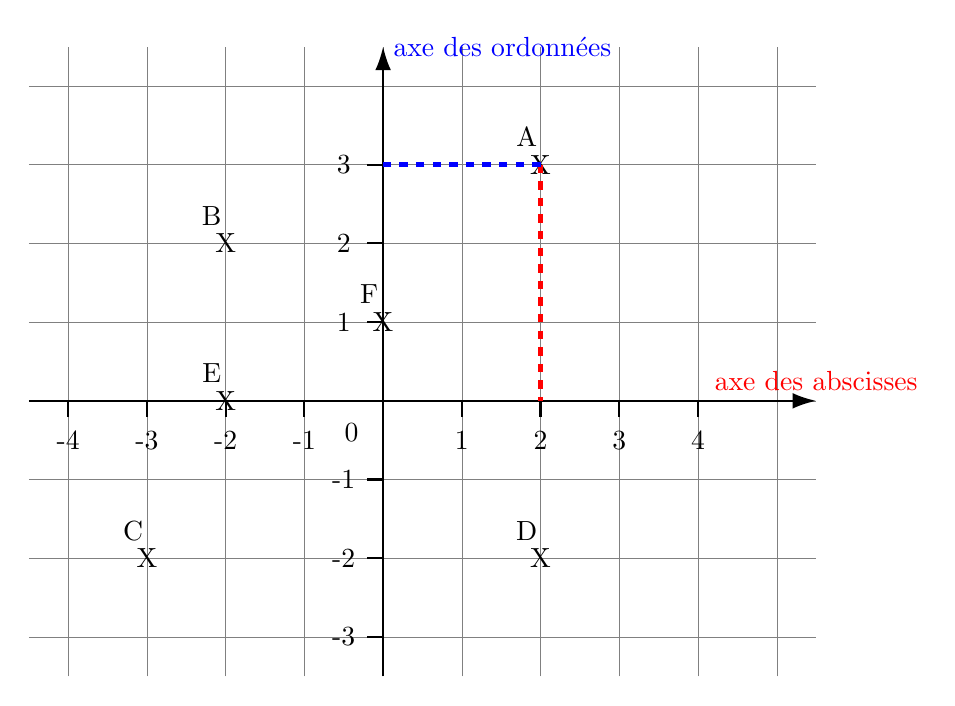
\begin{tikzpicture}
			\draw[ultra thin,gray] (-4.5,-3.5) grid (5.5,4.5);

			\draw[thick,-{Latex[length=3mm, width=2mm]}] (-4.5,0) -- (5.5,0) node[above] {\color{red} axe des abscisses};
			\draw[thick,-{Latex[length=3mm, width=2mm]}] (0,-3.5) -- (0,4.5) node[right] {\color{blue} axe des ordonnées};

			\foreach \x in {-4,...,-1,1,2,3,4} {
					\draw[thick] (\x,0) -- (\x,-0.2);
					\node at (\x,-0.5) {\x};
				}

			\foreach \y in {-3,...,-1,1,2,3} {
					\draw[thick] (0,\y) -- (-0.2,\y);
					\node at (-0.5,\y) {\y};
				}

			\coordinate (Origine) at (0,0);
			\node at (-0.4,-0.4) {0};

			\foreach \name \x \y in {A/2/3,B/-2/2,C/-3/-2,D/2/-2,E/-2/0,F/0/1} {
					\coordinate (\name) at (\x,\y);
					\node at (\x,\y) {X};
					\coordinate (\name-abscisse) at (\x,0);
					\coordinate (\name-ordonnée) at (0,\y);
					\node at ([yshift=1em,xshift=-0.5em] \name) {\name};
				}

			\draw[red,dashed,ultra thick] (A) -- (A-abscisse);
			\draw[blue,dashed,ultra thick] (A) -- (A-ordonnée);
		\end{tikzpicture}

		\begin{itemize}
			\item Le point A a pour coordonnées ({\color{red} 2}\hspace{0.6em} ; {\color{blue} 3} \hspace{0.1em}).
			\item Le point B a pour coordonnées (....;....).
			\item Le point C a pour coordonnées (....;....).
			\item Le point D a pour coordonnées (....;....).
			\item Le point E a pour coordonnées (....;....).
			\item Le point F a pour coordonnées (....;....).
		\end{itemize}
	\end{exemple}
}

\newpage
\Paste{Exemple}

\end{document}